
\chapter{Comparison to MD simulation\label{chpt:ions}}

In the last chapter, we proved that \acs{MDFT} is capable of
correctly predicting solvation properties of LJ centers, single ions
and linear solutes compared to \acs{IET}. In this section, we will
compare them to \acs{MD} and experimental results. All the solutes
are optimized with the fast \texttt{\textbf{convolution\_standard}}
algorithm, with implicitly $L=24$ $\textrm{Å}$, $\mathrm{nfft}=72$,
$m_{\max}=n_{\max}$ unless otherwise specified. Comparison to the
dipole method is also involved, as we should justify that the increase
of computing cost when going from $n_{\max}=1$ to $n_{\max}>1$ is
counterbalanced by the ability to produce better results. 

\section{LJ centers}

The \acs{RDF}s of rare gases calculated in $\mathsection$\ref{tab:Free-energy-rare-gas}
are compared to \acs{MD} in figure \ref{fig:rare-gazz} using $n_{\max}=3$
to 5. The structures of different $n_{\max}$ is almost identical.
Comparing to \acs{MD}, it seems there is no improvement over the dipole method 
in ref \citep{Zhao_2011} or to calculation involving
$c_{00}^{000}$ only \citep{levesque_scalar_2012}. This kind of disagreement
in curve shape is regarded as a known default of \acs{HNC} (or \acs{HRF})
approximation.

\begin{figure}[h]
\begin{centering}
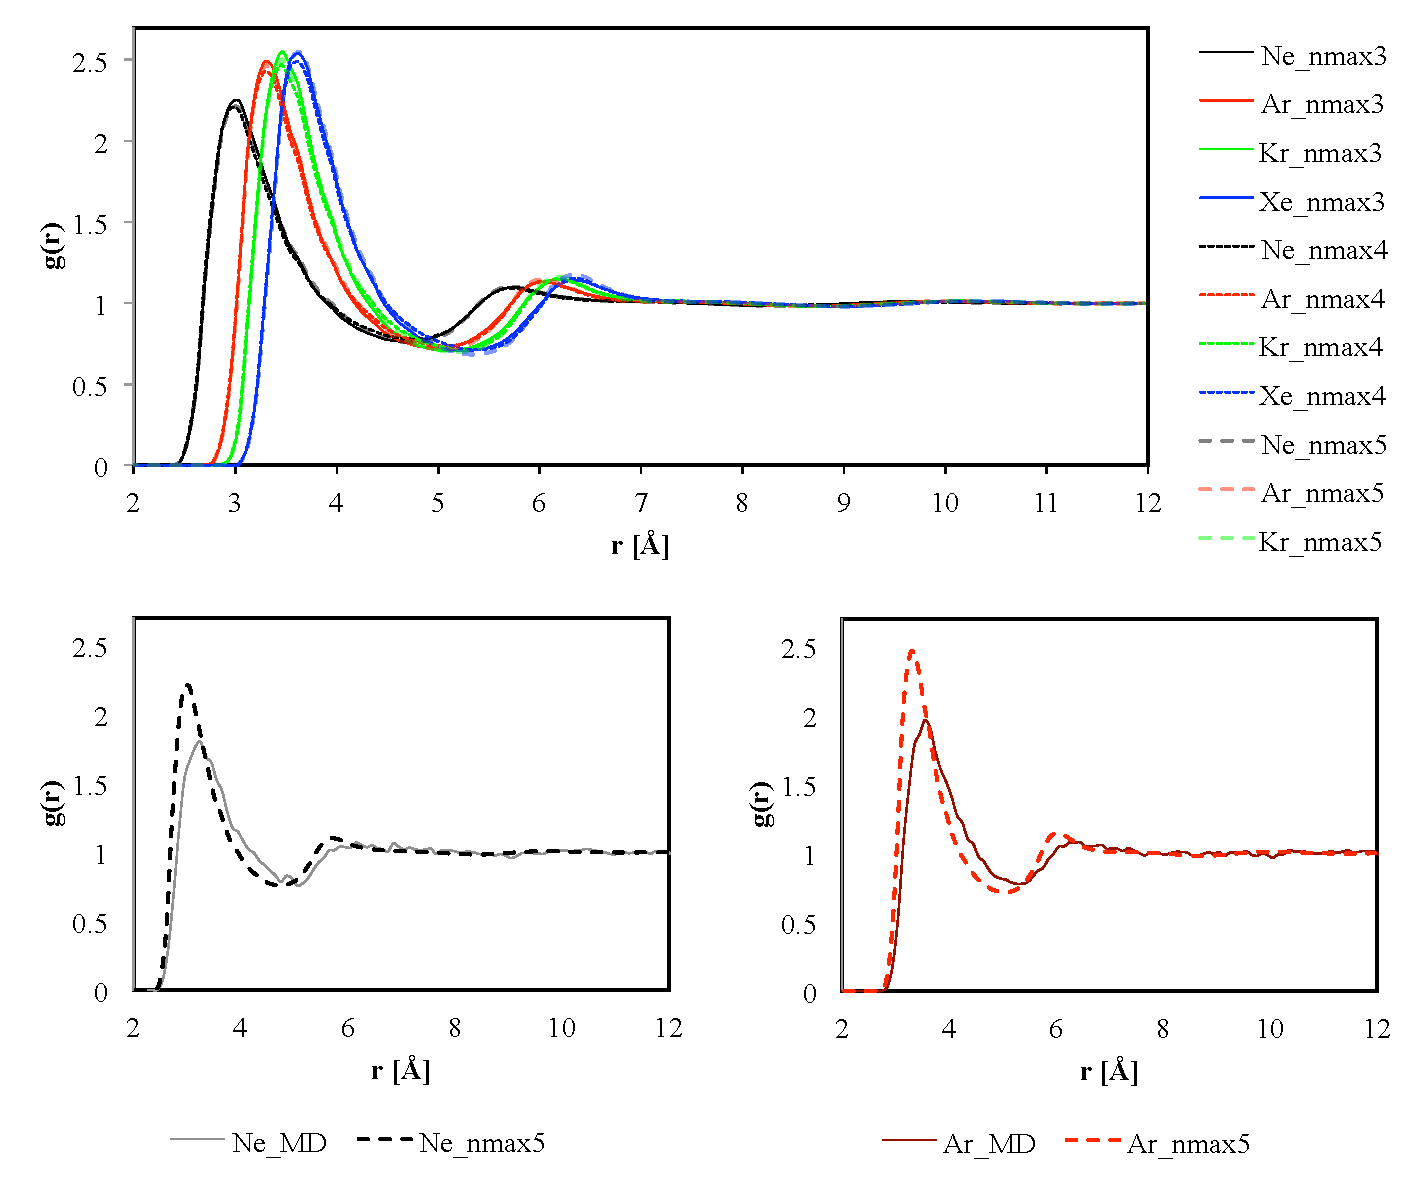
\includegraphics[width=0.95\columnwidth]{_figure/results/rare_gaz}
\par\end{centering}
\caption{\acs{RDF} of rare gasses compared to \acs{MD} result\label{fig:rare-gazz}}
\end{figure}


\section{Charged $\mathrm{CH_{4}}$ series}

The comparison between the \acs{RDF}s obtained from \acs{MDFT} with
\acs{MD} results for charged $\mathrm{CH_{4}}$ series are shown
in figure \ref{fig:Comparison-to-MD}. We can see that for positive
charges, the complete $n_{\max}=5$ gives much better results compared
to the dipole method, which itself almost agrees with \acs{MD} results.
For negative charges, $n_{\max}=5$ gives nearly the same result as
dipole method, while the \acs{MD} results are more smooth. Still the
first peak of the \acs{MDFT} results seems to be in a good position.
We can conclude that the complete \acs{DCF} gives a large improvement
for positive charged ions.

\begin{figure}[h]
\begin{centering}
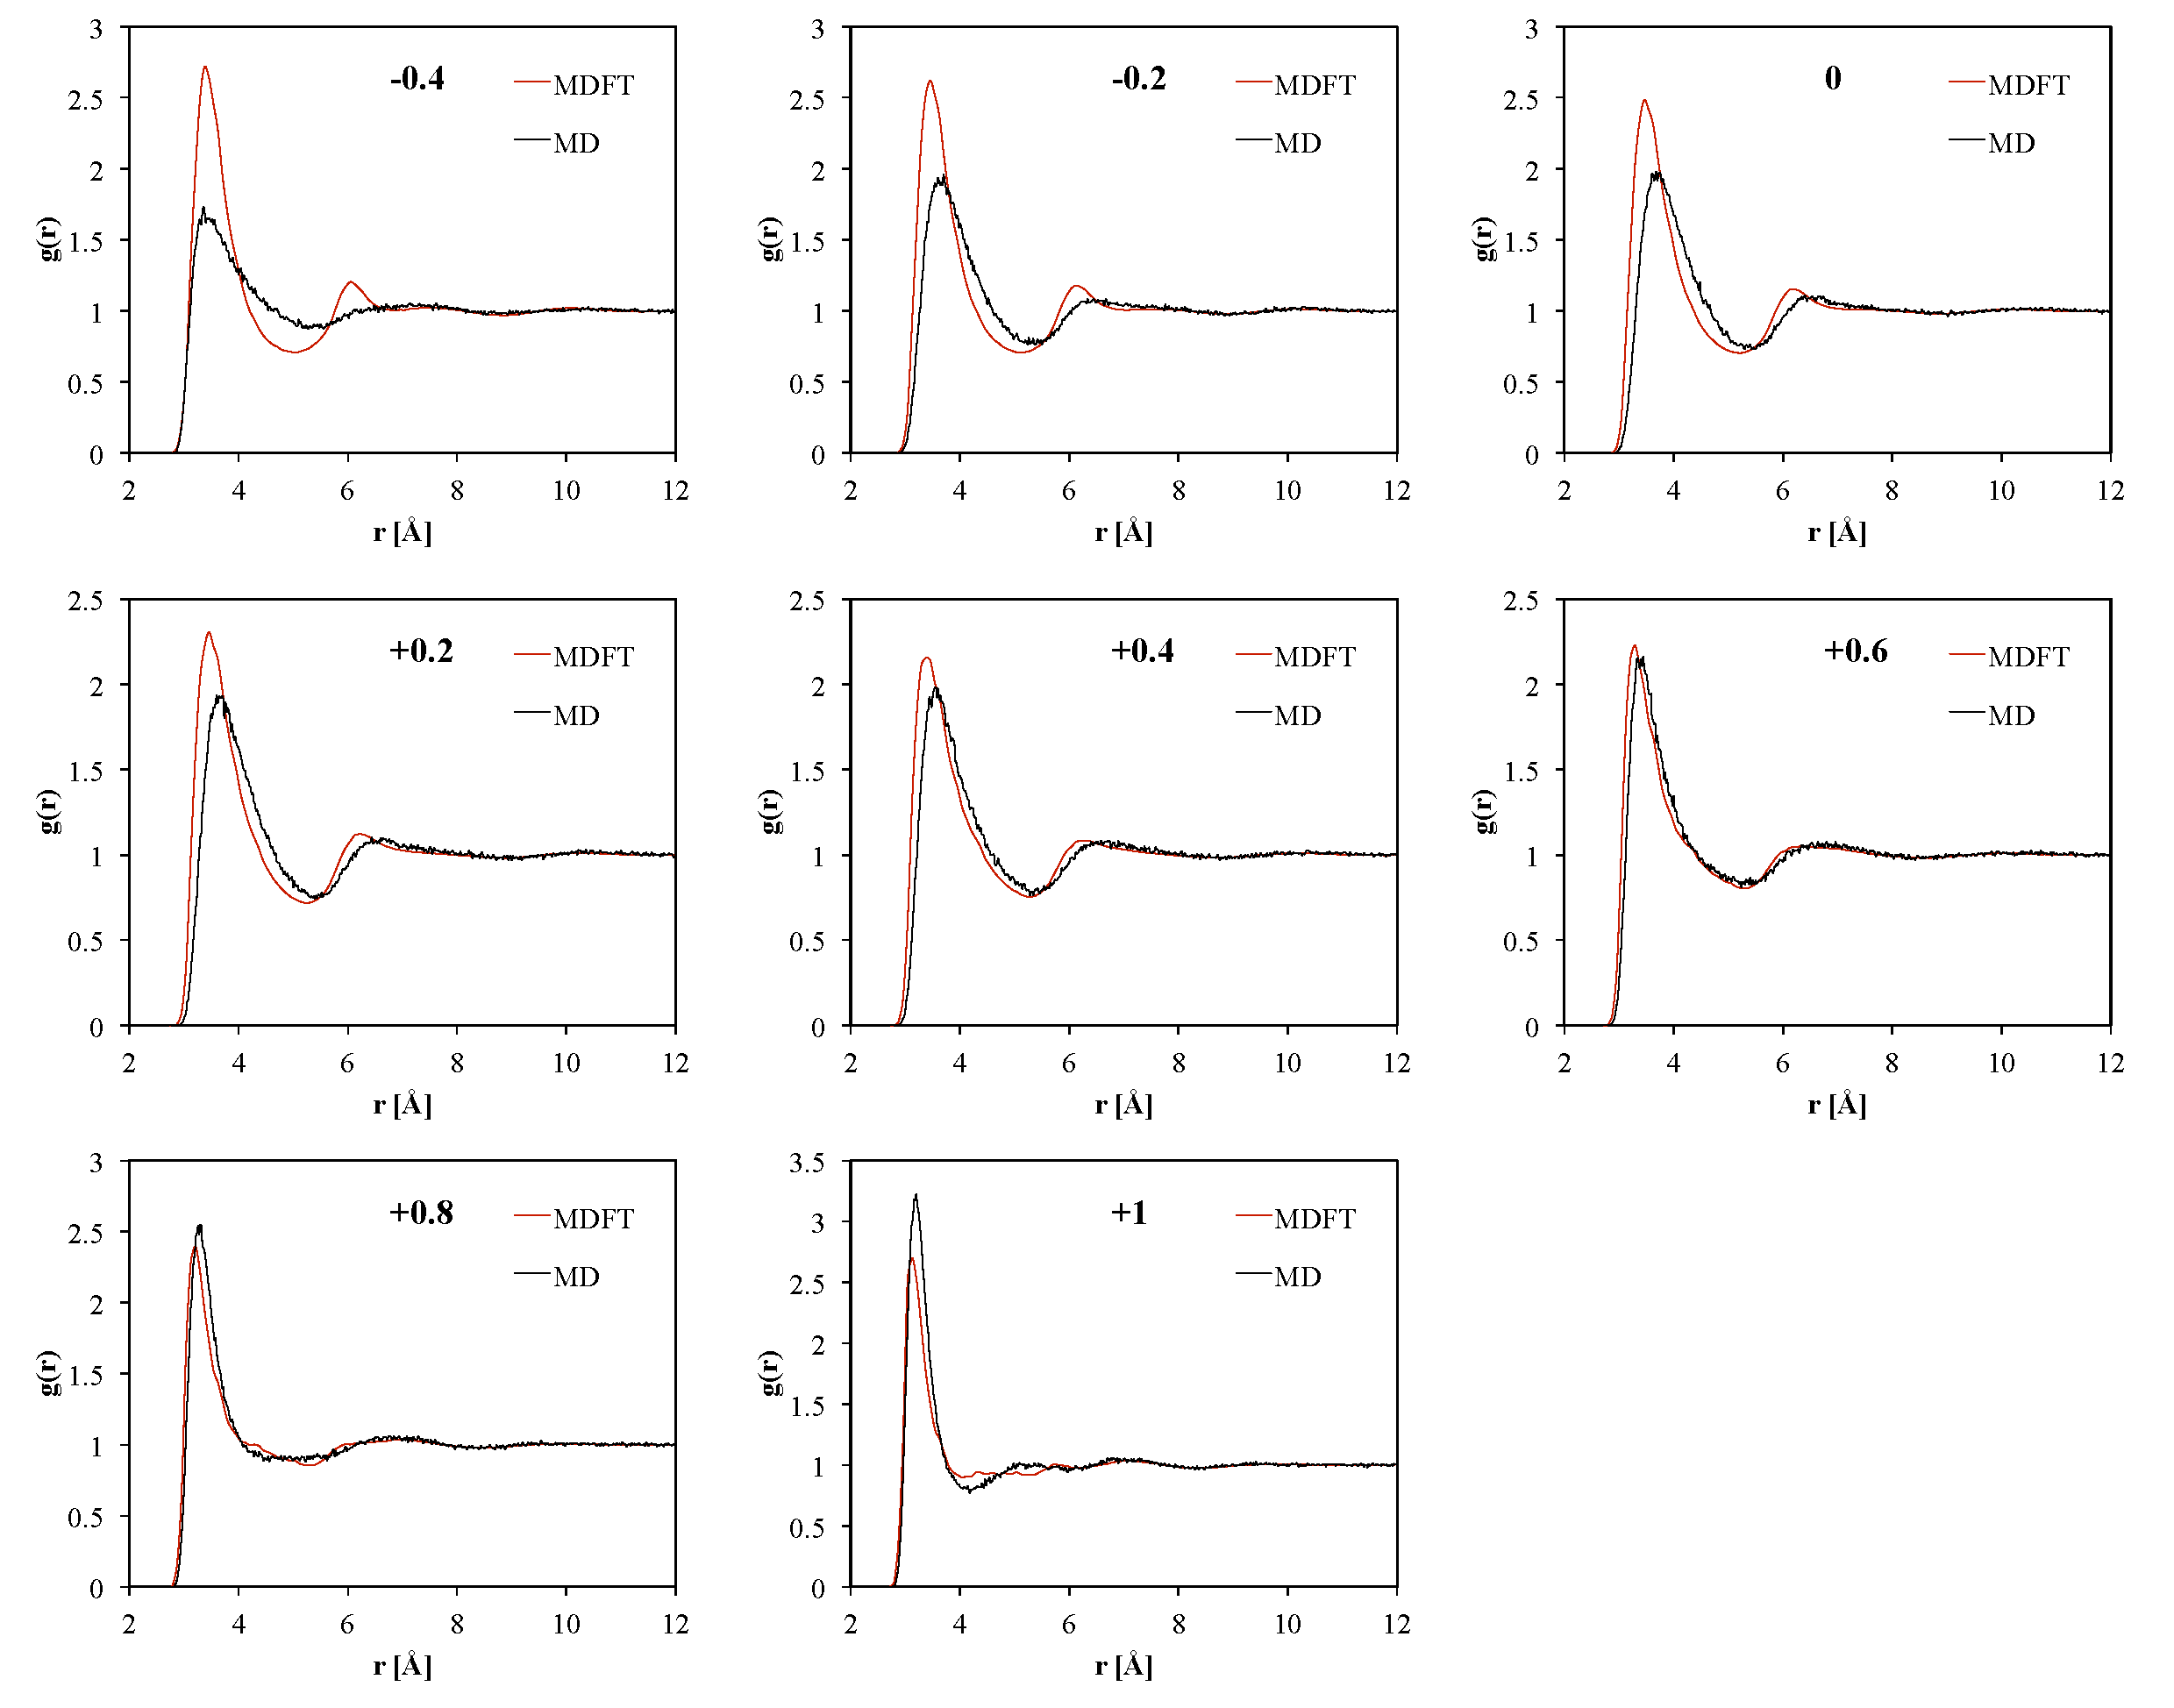
\includegraphics[width=1\columnwidth]{_figure/results/ch4_md}
\par\end{centering}
\caption{\acs{RDF} of charged $\mathrm{CH_{4}}$ series compared to \acs{MD}
result\label{fig:Comparison-to-MD}}
\end{figure}


\section{Solvation free energy of single ions}

\marginpar{We consider that in a macroscopic system, the fluctuation of $N$
and $V$ are negligible, and all kinds of free energies become the
same. \citep{ensemble_thermo}}From the previous paragraph we can see the \acs{RDF} for positive ions are in good
agreement with \acs{MD} results. However, the free energy is more
difficult to compare, as there are several finite-size corrections
for single ions, depending on for example box length and charge; besides,
the free energy depends largely on the input LJ parameters of the
ions, which is independent to the method.

Table \ref{tab:single-ions} gives some independent experimental
and \acs{MD} simulation results of solvation free energy as well
as the positions of the first maximum of the \acs{RDF} for alkali
and halide ions. We can see that the experimental data themselves
vary a lot. Furthermore the LJ parameters for ions in the literature
are extremely dispersed. Therefore, we focused on a single series
of force field parameters for halide anions and alkali cations taken
from ref \citep{horinek_rational_2009} based on SPC/E water, as shown
in table \ref{tab:single-ions}. 

\begin{table}[h]
\begin{centering}
\begin{tabular*}{1\linewidth}{@{\extracolsep{\fill}}ccccccccc}
\toprule 
\addlinespace[-0.17em]
\tableheadline{{\footnotesize{}Ion}} & {\scriptsize{}$-\Delta G_{\mathrm{solv}}^{\mathrm{exp}}$\textsuperscript{{\scriptsize{}(a)}}} & {\scriptsize{}$-\Delta F_{\mathrm{solv}}^{\mathrm{exp}}$\textsuperscript{{\scriptsize{}(b)}}} & {\scriptsize{}$-\Delta G_{\mathrm{solv}}^{\mathrm{exp}}$\textsuperscript{{\scriptsize{}(c)}}} & {\scriptsize{}$R_{1}$\textsuperscript{{\scriptsize{}(d)}}} & {\scriptsize{}$\sigma$ $[\textrm{Å}]$\textsuperscript{{\scriptsize{}(e)}}} & {\scriptsize{}$\epsilon$ {[}$\mathrm{kJ\cdot mol^{-1}}${]}\textsuperscript{{\scriptsize{}(e)}}} & {\scriptsize{}$-\Delta G_{\mathrm{solv}}^{\mathrm{MD}}$\textsuperscript{{\scriptsize{}(e)}}} & {\scriptsize{}$R_{1}^{\mathrm{MD}}$\textsuperscript{{\scriptsize{}(e)}}}\tabularnewline
\midrule 
\addlinespace[-0.33em]
{\scriptsize{}$\mathrm{F^{-}}$} & {\scriptsize{}465} & {\scriptsize{}374.5} & {\scriptsize{}428.8} & {\scriptsize{}2.08} & {\scriptsize{}3.30} & {\scriptsize{}0.55} & {\scriptsize{}-430} & {\scriptsize{}2.74}\tabularnewline
\addlinespace[-0.33em]
{\scriptsize{}$\mathrm{Cl^{-}}$} & {\scriptsize{}340} & {\scriptsize{}318.4} & {\scriptsize{}304.2} & {\scriptsize{}2.36} & {\scriptsize{}3.78} & {\scriptsize{}0.52} & {\scriptsize{}-306} & {\scriptsize{}3.23}\tabularnewline
\addlinespace[-0.33em]
{\scriptsize{}$\mathrm{Br^{-}}$} & {\scriptsize{}315} & {\scriptsize{}289.5} & {\scriptsize{}227.4} & {\scriptsize{}2.80} & {\scriptsize{}4.00} & {\scriptsize{}0.37} & {\scriptsize{}-279} & {\scriptsize{}3.35}\tabularnewline
\addlinespace[-0.33em]
{\scriptsize{}$\mathrm{I^{-}}$ } & {\scriptsize{}275} & {\scriptsize{}252.3} & {\scriptsize{}240.0} & {\scriptsize{}2.89} & {\scriptsize{}4.25} & {\scriptsize{}0.32} & {\scriptsize{}-241} & {\scriptsize{}3.55}\tabularnewline
\addlinespace[-0.33em]
{\scriptsize{}$\mathrm{Li^{+}}$ } & {\scriptsize{}475} & {\scriptsize{}511.0} & {\scriptsize{}529.4} & {\scriptsize{}3.14} & {\scriptsize{}3.02} & {\scriptsize{}0.02} & {\scriptsize{}-520} & {\scriptsize{}1.91}\tabularnewline
\addlinespace[-0.33em]
{\scriptsize{}$\mathrm{Na^{+}}$ } & {\scriptsize{}365} & {\scriptsize{}411.5} & {\scriptsize{}423.8} & {\scriptsize{}2.63} & {\scriptsize{}3.49} & {\scriptsize{}0.02} & {\scriptsize{}-414} & {\scriptsize{}2.28}\tabularnewline
\addlinespace[-0.33em]
{\scriptsize{}$\mathrm{K^{+}}$ } & {\scriptsize{}295} & {\scriptsize{}337.2} & {\scriptsize{}352.0} & {\scriptsize{}3.19} & {\scriptsize{}3.85} & {\scriptsize{}0.02} & {\scriptsize{}-347} & {\scriptsize{}2.54}\tabularnewline
\addlinespace[-0.33em]
{\scriptsize{}$\mathrm{Rb^{+}}$ } & {\scriptsize{}275} & {\scriptsize{}316.0} & {\scriptsize{}329.3} & {\scriptsize{}3.37} & {\scriptsize{}no data} & {\scriptsize{}no data} & {\scriptsize{}no data} & {\scriptsize{}no data}\tabularnewline
\addlinespace[-0.33em]
{\scriptsize{}$\mathrm{Cs^{+}}$ } & {\scriptsize{}250} & {\scriptsize{}283.8} & {\scriptsize{}no data} & {\scriptsize{}3.65} & {\scriptsize{}4.17} & {\scriptsize{}0.02} & {\scriptsize{}-300} & {\scriptsize{}2.79}\tabularnewline
\bottomrule
\end{tabular*}
\par\end{centering}
\caption[Free energy and first maximum of ion-water oxygen \acs{RDF} for alkali
and halide ions from experimental and \acs{MD} simulation results]{Free energy $[\mathrm{kJ\cdot mol^{-1}}]$ and first maximum of ion-water
oxygen \acs{RDF} $[\textrm{Å}]$ for alkali and halide ions from
experimental and \acs{MD} simulation result. (a). Ref \citep{MARCUS1994111}.
(b). Ref \citep{Noyes_1962}. (c) Ref \citep{tissandier_protons_1998}.
(e) Ref \citep{horinek_rational_2009} from \acs{MD} simulation.
(d) Ref \citep{Marcus_1988}.\label{tab:single-ions}}

\vspace{0.5cm}

\begin{centering}
\begin{tabular*}{1\linewidth}{@{\extracolsep{\fill}}ccccccc}
\toprule 
\addlinespace[-0.17em]
\tableheadline{{\footnotesize{}Ion}} & {\scriptsize{}$\Delta G_{\mathrm{solv}}^{\mathrm{MD}}$} & {\scriptsize{}$\Delta\varOmega_{\mathrm{solv}}^{\mathrm{dipole}}$} & {\scriptsize{}$\Delta\varOmega_{\mathrm{solv}}^{\mathrm{nmax3}}$} & {\scriptsize{}$R_{1}^{\mathrm{MD}}$} & {\scriptsize{}$R_{1}^{\mathrm{dipole}}$} & {\scriptsize{}$R_{1}^{\mathrm{nmax3}}$}\tabularnewline
\midrule 
\addlinespace[-0.33em]
{\scriptsize{}$\mathrm{F^{-}}$ } & {\scriptsize{}-430} & {\scriptsize{}diverge} & {\scriptsize{}-368.5} & {\scriptsize{}2.74} & {\scriptsize{}-} & {\scriptsize{}2.71}\tabularnewline
\addlinespace[-0.33em]
{\scriptsize{}$\mathrm{Cl^{-}}$ } & {\scriptsize{}-306} & {\scriptsize{}diverge} & {\scriptsize{}-297.3} & {\scriptsize{}3.23} & {\scriptsize{}-} & {\scriptsize{}2.88}\tabularnewline
\addlinespace[-0.33em]
{\scriptsize{}$\mathrm{Br^{-}}$ } & {\scriptsize{}-279} & {\scriptsize{}diverge} & {\scriptsize{}-278.3} & {\scriptsize{}3.35} & {\scriptsize{}-} & {\scriptsize{}2.96}\tabularnewline
\addlinespace[-0.33em]
{\scriptsize{}$\mathrm{I^{-}}$ } & {\scriptsize{}-241} & {\scriptsize{}diverge} & {\scriptsize{}-253.4} & {\scriptsize{}3.55} & {\scriptsize{}-} & {\scriptsize{}3.12}\tabularnewline
\addlinespace[-0.33em]
{\scriptsize{}$\mathrm{Li^{+}}$ } & {\scriptsize{}-520} & {\scriptsize{}-707.7} & {\scriptsize{}-405.3} & {\scriptsize{}1.91} & {\scriptsize{}2.46} & {\scriptsize{}2.38}\tabularnewline
\addlinespace[-0.33em]
{\scriptsize{}$\mathrm{Na^{+}}$ } & {\scriptsize{}-414} & {\scriptsize{}-621.8} & {\scriptsize{}-366.0} & {\scriptsize{}2.28} & {\scriptsize{}2.54} & {\scriptsize{}2.54}\tabularnewline
\addlinespace[-0.33em]
{\scriptsize{}$\mathrm{K^{+}}$ } & {\scriptsize{}-347} & {\scriptsize{}-559.1} & {\scriptsize{}-338.4} & {\scriptsize{}2.54} & {\scriptsize{}2.63} & {\scriptsize{}2.70}\tabularnewline
\addlinespace[-0.33em]
{\scriptsize{}$\mathrm{Cs^{+}}$ } & {\scriptsize{}-300} & {\scriptsize{}-508.8} & {\scriptsize{}-316.1} & {\scriptsize{}2.79} & {\scriptsize{}2.88} & {\scriptsize{}2.88}\tabularnewline
\bottomrule
\end{tabular*}
\par\end{centering}
\caption[Free energies and first \acs{RDF} maximum of single ions from \acs{MDFT}
results]{Free energies $[\mathrm{kJ\cdot mol^{-1}}]$ and first \acs{RDF}
maximum $[\textrm{Å}]$ of single ions from \acs{MDFT} results compared
to \acs{MD} results \label{tab:free-energy-single-ions}}
\end{table}

The results shows that the free energies given by \acs{MDFT} are not
perfect, but lie in the same order of magnitude as \acs{MD} for $\mathrm{Cl}^{-}$
to $\mathrm{I}^{-}$ and $\mathrm{K}^{+}$ to $\mathrm{Cs}^{+}$.
They are much less convincing for small ions such as $\mathrm{F}^{-}$,
$\mathrm{Li}^{+}$ and $\mathrm{Na}^{+}$. Besides, the results with
a \acs{DCF} at $n_{\max}=3$ work better than the dipolar approximation,
which is a positive sign for our developments. In contrast, there
is no improvement in terms of position of the first solvation maximum.
Note that for this quantity, the agreement between experimental data
and \acs{MD} is not obvious either. 

\section{Small molecules}

\acs{MDFT} calculations involving some small molecular solutes were
also generated to compare to \acs{MD}; the chosen solutes are shown
in figure \ref{fig:Test-solutes-2} and defined in table \ref{tab:Parameters-of-test-solutes-2}.
Note that a certain proportion of them have a non-linear, 3-dimensional
geometry which could not be handled by the molecular \acs{IET}; this
shows the advantage of the general 3D-\acs{MDFT} approach adopted
in this thesis and the new algorithm that we have developed in this
context.

Figure \ref{fig:Site-O} gives the site-site \acs{RDF}s (solute site
to water O site) for $n_{\max}=4$, the dipolar approximation ($n_{\max}=1$),
and \acs{MD} for these test solutes. It is shown that in most
of the cases, $n_{\max}=4$ does give equivalent or better results
than the dipolar order, apart from the cases of water, and especially
SPC/E water. In methanol, the dipole method diverges. For most solutes,
the comparison to \acs{MD} is far from perfect but can be qualified
as satisfactory in reproducing the - sometimes complex - shape of
the \acs{RDF}s and the main peaks positions. This statement is especially
true for benzene and pyrimidine, for example. For hydrophobic molecules
or molecules with hydrophobic sites (alkanes, oxygen, nitrogen)
one recovers the slight underestimation of the first peak position
and the overestimation of peak height already remarked for
rare gases; this is a clear defect of \acs{HNC}. The case of molecules
giving rise to hydrogen bonds to water (e.g. methanol, or water in
water) is more problematic and subtle. Here the dipolar approximation
gives a first peak for the water oxygen around the O-site that is
too high but has the correct width, whereas $n_{\max}=4$ shifts the
first peak to higher values and makes it too wide (a sort of merge
of the first and second peak, an effect even clearer for methanol).
The H-O first peak, on the other hand, is at a correct position but
underestimated, both for water and methanol. The tetrahedral order
around a water solute is not correctly reproduced, although the correct
balance to get the right structure is subtle and does not appear too
far. 

For the purpose of showing the ability of \acs{MDFT} to calculate
3D solute structure, we display 3D solvent densities for specific
solutes in figure \ref{fig:Volume-slice-of} and \ref{fig:Iso-surface-of-solvent}.
Figure \ref{fig:Iso-surface-of-solvent} complements the discussion
given just above concerning the expected tetrahedral structure around
a water molecule in water. That structure can indeed be detected for
SPC/E water and even more so for the TIP4P model. In SPC/E water,
there is more density than expected on the north pole, and this piece
of density disappears with the extra charge added on the TIP4P water.\\

\begin{figure}[H]
\begin{centering}
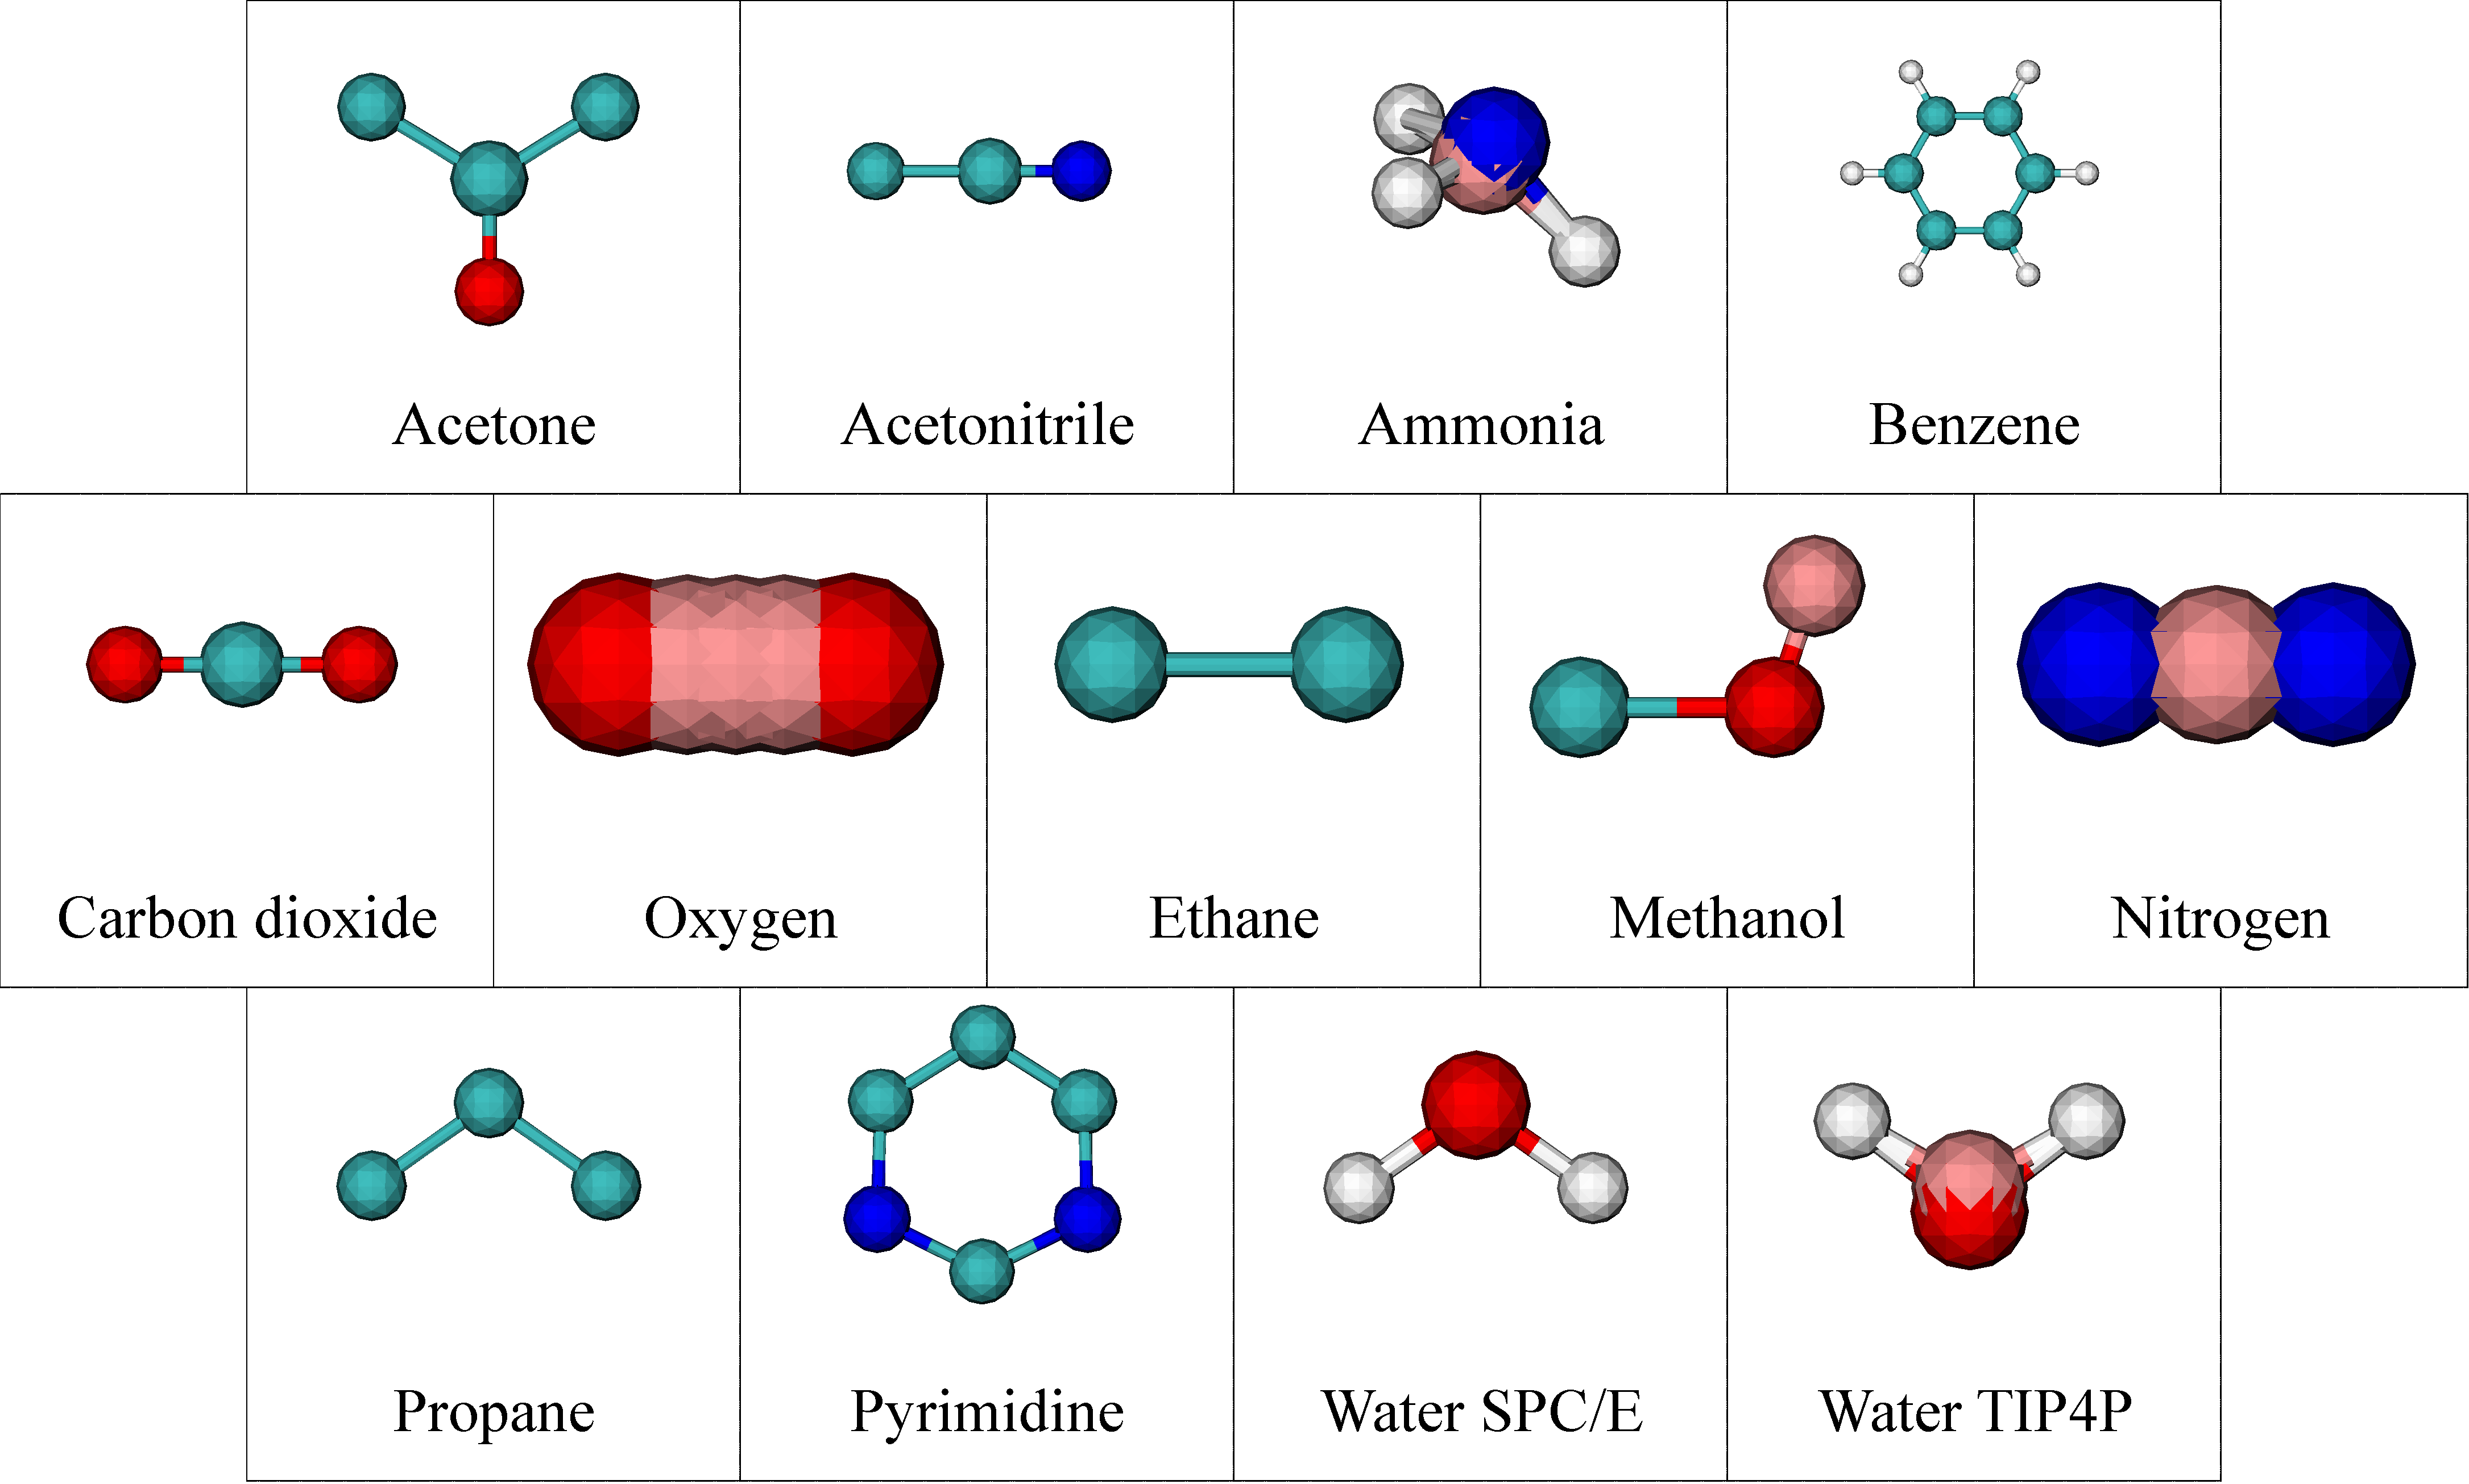
\includegraphics[width=1\columnwidth]{_figure/app_solute_var}
\par\end{centering}
\caption{Test solutes\label{fig:Test-solutes-2}}
\end{figure}

\begin{table}[H]
\begin{centering}
\begin{tabular*}{1\linewidth}{@{\extracolsep{\fill}}llrrrrrr}
\toprule 
\addlinespace[-0.17em]
\tableheadline{{\footnotesize{}Solute}} & \tableheadline{{\footnotesize{}Site}} & {\scriptsize{}$q$} & {\scriptsize{}$\sigma$ $[\textrm{Å}]$} & {\scriptsize{}$\epsilon$ {[}$\mathrm{kJ\cdot mol^{-1}}${]}} & {\scriptsize{}$x$ $[\textrm{Å}]$} & {\scriptsize{}$y$ $[\textrm{Å}]$} & {\scriptsize{}$z$ $[\textrm{Å}]$}\tabularnewline
\midrule 
\addlinespace[-0.33em]
{\scriptsize{}Acetone \citep{jorgensen_relative_1990}} & {\scriptsize{}CH\textsubscript{3}} & {\scriptsize{}0.062} & {\scriptsize{}3.91} & {\scriptsize{}0.6694} & {\scriptsize{}1.2810} & {\scriptsize{}0.7024} & {\scriptsize{}-0.0002}\tabularnewline
\addlinespace[-0.17em]
\addlinespace[-0.33em]
 & {\scriptsize{}C} & {\scriptsize{}0.300} & {\scriptsize{}3.75} & {\scriptsize{}0.4393} & {\scriptsize{}0.0101} & {\scriptsize{}-0.0872 } & {\scriptsize{}0.0106 }\tabularnewline
\addlinespace[-0.17em]
\addlinespace[-0.33em]
 & {\scriptsize{}O} & {\scriptsize{}-0.424} & {\scriptsize{}2.96} & {\scriptsize{}0.8796} & {\scriptsize{}0.0103} & {\scriptsize{}-1.3171 } & {\scriptsize{}-0.0102 }\tabularnewline
\addlinespace[-0.17em]
\addlinespace[-0.33em]
 & {\scriptsize{}CH\textsubscript{3}} & {\scriptsize{}0.062} & {\scriptsize{}3.91} & {\scriptsize{}0.6694} & {\scriptsize{}-1.2813} & {\scriptsize{}0.7019} & {\scriptsize{}-0.0002}\tabularnewline
\addlinespace[-0.17em]
\midrule 
\addlinespace[-0.33em]
{\scriptsize{}Acetonitrile }\textcolor{red}{\scriptsize{}{[}ref{]}} & {\scriptsize{}CH\textsubscript{3}} & {\scriptsize{}0.269 } & {\scriptsize{}3.6 } & {\scriptsize{}1.590 } & {\scriptsize{}0.0000} & {\scriptsize{}0.0000} & {\scriptsize{}-1.3254 }\tabularnewline
\addlinespace[-0.17em]
\addlinespace[-0.33em]
 & {\scriptsize{}C} & {\scriptsize{}0.129} & {\scriptsize{}3.4 } & {\scriptsize{}0.416 } & {\scriptsize{}0.0000} & {\scriptsize{}0.0000} & {\scriptsize{}0.1346}\tabularnewline
\addlinespace[-0.17em]
\addlinespace[-0.33em]
 & {\scriptsize{}N} & {\scriptsize{}-0.398 } & {\scriptsize{}3.3 } & {\scriptsize{}0.416 } & {\scriptsize{}0.0000} & {\scriptsize{}0.0000} & {\scriptsize{}1.3046}\tabularnewline
\addlinespace[-0.17em]
\midrule 
\addlinespace[-0.33em]
{\scriptsize{}Ammonia \citep{Diraison_1999}} & {\scriptsize{}N} & {\scriptsize{}0.000 } & {\scriptsize{}3.4 } & {\scriptsize{}1.164 } & {\scriptsize{}0.000000} & {\scriptsize{}0.000000} & {\scriptsize{}0.000000}\tabularnewline
\addlinespace[-0.17em]
\addlinespace[-0.33em]
 & {\scriptsize{}X} & {\scriptsize{}-1.386} & {\scriptsize{}0.0} & {\scriptsize{}0.000} & {\scriptsize{}0.000000} & {\scriptsize{}0.000000} & {\scriptsize{}-0.156000}\tabularnewline
\addlinespace[-0.17em]
\addlinespace[-0.33em]
 & {\scriptsize{}H} & {\scriptsize{}0.462} & {\scriptsize{}0.0} & {\scriptsize{}0.000} & {\scriptsize{}-0.937790} & {\scriptsize{}0.000000} & {\scriptsize{}-0.381449}\tabularnewline
\addlinespace[-0.17em]
\addlinespace[-0.33em]
 & {\scriptsize{}H} & {\scriptsize{}0.462} & {\scriptsize{}0.0} & {\scriptsize{}0.000} & {\scriptsize{}0.468895} & {\scriptsize{}0.812150} & {\scriptsize{}-0.381449}\tabularnewline
\addlinespace[-0.17em]
\addlinespace[-0.33em]
 & {\scriptsize{}H} & {\scriptsize{}0.462} & {\scriptsize{}0.0} & {\scriptsize{}0.000} & {\scriptsize{}0.468895} & {\scriptsize{}-0.812150} & {\scriptsize{}-0.381449}\tabularnewline
\addlinespace[-0.17em]
\midrule 
\addlinespace[-0.33em]
{\scriptsize{}Benzene \citep{Chipot_1996}} & {\scriptsize{}C} & {\scriptsize{}-0.138} & {\scriptsize{}1.908 } & {\scriptsize{}0.35980 } & {\scriptsize{}1.386 } & {\scriptsize{}0.000} & {\scriptsize{}0.000}\tabularnewline
\addlinespace[-0.17em]
\addlinespace[-0.33em]
{\scriptsize{}(charged)} & {\scriptsize{}C} & {\scriptsize{}-0.138} & {\scriptsize{}1.908 } & {\scriptsize{}0.35980 } & {\scriptsize{}0.693} & {\scriptsize{}-1.200} & {\scriptsize{}0.000}\tabularnewline
\addlinespace[-0.17em]
\addlinespace[-0.33em]
 & {\scriptsize{}C} & {\scriptsize{}-0.138} & {\scriptsize{}1.908 } & {\scriptsize{}0.35980 } & {\scriptsize{}-0.693} & {\scriptsize{}-1.200} & {\scriptsize{}0.000}\tabularnewline
\addlinespace[-0.17em]
\addlinespace[-0.33em]
 & {\scriptsize{}C} & {\scriptsize{}-0.138} & {\scriptsize{}1.908 } & {\scriptsize{}0.35980 } & {\scriptsize{}-1.386} & {\scriptsize{}0.000} & {\scriptsize{}0.000}\tabularnewline
\addlinespace[-0.17em]
\addlinespace[-0.33em]
 & {\scriptsize{}C} & {\scriptsize{}-0.138} & {\scriptsize{}1.908 } & {\scriptsize{}0.35980 } & {\scriptsize{}-0.693} & {\scriptsize{}1.200} & {\scriptsize{}0.000}\tabularnewline
\addlinespace[-0.17em]
\addlinespace[-0.33em]
 & {\scriptsize{}C} & {\scriptsize{}-0.138} & {\scriptsize{}1.908 } & {\scriptsize{}0.35980 } & {\scriptsize{}0.693} & {\scriptsize{}1.200} & {\scriptsize{}0.000}\tabularnewline
\addlinespace[-0.17em]
\addlinespace[-0.33em]
 & {\scriptsize{}H} & {\scriptsize{}0.138 } & {\scriptsize{}1.459} & {\scriptsize{}0.06276 } & {\scriptsize{}2.462} & {\scriptsize{}0.000} & {\scriptsize{}0.000}\tabularnewline
\addlinespace[-0.17em]
\addlinespace[-0.33em]
 & {\scriptsize{}H} & {\scriptsize{}0.138 } & {\scriptsize{}1.459} & {\scriptsize{}0.06276 } & {\scriptsize{}1.231} & {\scriptsize{}-2.132} & {\scriptsize{}0.000}\tabularnewline
\addlinespace[-0.17em]
\addlinespace[-0.33em]
 & {\scriptsize{}H} & {\scriptsize{}0.138 } & {\scriptsize{}1.459} & {\scriptsize{}0.06276 } & {\scriptsize{}-1.231} & {\scriptsize{}-2.132} & {\scriptsize{}0.000}\tabularnewline
\addlinespace[-0.17em]
\addlinespace[-0.33em]
 & {\scriptsize{}H} & {\scriptsize{}0.138 } & {\scriptsize{}1.459} & {\scriptsize{}0.06276 } & {\scriptsize{}-2.462} & {\scriptsize{}0.000} & {\scriptsize{}0.000}\tabularnewline
\addlinespace[-0.17em]
\addlinespace[-0.33em]
 & {\scriptsize{}H} & {\scriptsize{}0.138 } & {\scriptsize{}1.459} & {\scriptsize{}0.06276 } & {\scriptsize{}-1.231} & {\scriptsize{}2.132} & {\scriptsize{}0.000}\tabularnewline
\addlinespace[-0.17em]
\addlinespace[-0.33em]
 & {\scriptsize{}H} & {\scriptsize{}0.138 } & {\scriptsize{}1.459} & {\scriptsize{}0.06276 } & {\scriptsize{}1.231} & {\scriptsize{}2.132} & {\scriptsize{}0.000}\tabularnewline
\addlinespace[-0.17em]
\midrule 
\addlinespace[-0.33em]
{\scriptsize{}$\mathrm{CO_{2}}$ \citep{Harris_1995}} & {\scriptsize{}C} & {\scriptsize{}0.6512 } & {\scriptsize{}2.76} & {\scriptsize{}0.234} & {\scriptsize{}0.000 } & {\scriptsize{}0.000 } & {\scriptsize{}0.000 }\tabularnewline
\addlinespace[-0.17em]
\addlinespace[-0.33em]
 & {\scriptsize{}O} & {\scriptsize{}-0.3256} & {\scriptsize{}3.03 } & {\scriptsize{}0.67} & {\scriptsize{}-1.149 } & {\scriptsize{}0.000 } & {\scriptsize{}0.000 }\tabularnewline
\addlinespace[-0.17em]
\addlinespace[-0.33em]
 & {\scriptsize{}O} & {\scriptsize{}-0.3256} & {\scriptsize{}3.03 } & {\scriptsize{}0.67} & {\scriptsize{}1.149 } & {\scriptsize{}0.000 } & {\scriptsize{}0.000 }\tabularnewline
\addlinespace[-0.17em]
\midrule 
\addlinespace[-0.33em]
{\scriptsize{}$\mathrm{O_{2}}$ \citep{Boutard200525}} & {\scriptsize{}O} & {\scriptsize{}0.0} & {\scriptsize{}3.1062} & {\scriptsize{}0.36 } & {\scriptsize{}-0.485} & {\scriptsize{}0.000 } & {\scriptsize{}0.000 }\tabularnewline
\addlinespace[-0.17em]
\addlinespace[-0.33em]
 & {\scriptsize{}O} & {\scriptsize{}0.0} & {\scriptsize{}3.1062} & {\scriptsize{}0.36 } & {\scriptsize{}0.485} & {\scriptsize{}0.000 } & {\scriptsize{}0.000 }\tabularnewline
\addlinespace[-0.17em]
\addlinespace[-0.33em]
 & {\scriptsize{}X} & {\scriptsize{}-2.1} & {\scriptsize{}0.00} & {\scriptsize{}0.00} & {\scriptsize{}-0.200} & {\scriptsize{}0.000 } & {\scriptsize{}0.000 }\tabularnewline
\addlinespace[-0.17em]
\addlinespace[-0.33em]
 & {\scriptsize{}X} & {\scriptsize{}-2.1} & {\scriptsize{}0.00} & {\scriptsize{}0.00} & {\scriptsize{}0.200} & {\scriptsize{}0.000 } & {\scriptsize{}0.000 }\tabularnewline
\addlinespace[-0.17em]
\addlinespace[-0.33em]
 & {\scriptsize{}X} & {\scriptsize{}4.2} & {\scriptsize{}0.00} & {\scriptsize{}0.00} & {\scriptsize{}0.000} & {\scriptsize{}0.000 } & {\scriptsize{}0.000 }\tabularnewline
\addlinespace[-0.17em]
\midrule 
\addlinespace[-0.33em]
{\scriptsize{}Ethane \citep{jorgensen_relative_1990}} & {\scriptsize{}CH\textsubscript{3}} & {\scriptsize{}0.0} & {\scriptsize{}3.775} & {\scriptsize{}0.8661} & {\scriptsize{}-0.756} & {\scriptsize{}0.000} & {\scriptsize{}0.000}\tabularnewline
\addlinespace[-0.17em]
\addlinespace[-0.33em]
 & {\scriptsize{}CH\textsubscript{3}} & {\scriptsize{}0.0} & {\scriptsize{}3.775} & {\scriptsize{}0.8661} & {\scriptsize{}0.756} & {\scriptsize{}0.000} & {\scriptsize{}0.000}\tabularnewline
\addlinespace[-0.17em]
\midrule 
\addlinespace[-0.33em]
{\scriptsize{}Methanol \citep{Schnabel_2007}} & {\scriptsize{}CH\textsubscript{3}} & {\scriptsize{}0.24746} & {\scriptsize{}3.7543} & {\scriptsize{}1.0027} & {\scriptsize{}-1.42460} & {\scriptsize{}0.000000} & {\scriptsize{}0.000000}\tabularnewline
\addlinespace[-0.17em]
\addlinespace[-0.33em]
 & {\scriptsize{}OH} & {\scriptsize{}-0.67874} & {\scriptsize{}3.0300} & {\scriptsize{}0.7307} & {\scriptsize{}0.00000} & {\scriptsize{}0.000000} & {\scriptsize{}0.000000}\tabularnewline
\addlinespace[-0.17em]
\addlinespace[-0.33em]
 & {\scriptsize{}X} & {\scriptsize{}0.43128} & {\scriptsize{}0.0000} & {\scriptsize{}0.0000} & {\scriptsize{}0.30035} & {\scriptsize{}0.896104} & {\scriptsize{}0.000000}\tabularnewline
\addlinespace[-0.17em]
\midrule 
\addlinespace[-0.33em]
{\scriptsize{}$\mathrm{N_{2}}$ }\textcolor{red}{\scriptsize{}{[}ref{]}} & {\scriptsize{}N} & {\scriptsize{}-0.5075} & {\scriptsize{}3.30} & {\scriptsize{}0.30} & {\scriptsize{}-0.549} & {\scriptsize{}0.000} & {\scriptsize{}0.000}\tabularnewline
\addlinespace[-0.17em]
\addlinespace[-0.33em]
 & {\scriptsize{}N} & {\scriptsize{}-0.5075} & {\scriptsize{}3.30} & {\scriptsize{}0.30} & {\scriptsize{}0.549} & {\scriptsize{}0.000} & {\scriptsize{}0.000}\tabularnewline
\addlinespace[-0.17em]
\addlinespace[-0.33em]
 & {\scriptsize{}X} & {\scriptsize{}1.0150} & {\scriptsize{}0.00} & {\scriptsize{}0.00} & {\scriptsize{}0.000} & {\scriptsize{}0.000} & {\scriptsize{}0.000}\tabularnewline
\addlinespace[-0.17em]
\midrule 
\addlinespace[-0.33em]
{\scriptsize{}Propane }\textcolor{red}{\scriptsize{}{[}ref{]}} & {\scriptsize{}CH\textsubscript{3}} & {\scriptsize{}0.0} & {\scriptsize{}3.905} & {\scriptsize{}0.732} & {\scriptsize{}-1.25} & {\scriptsize{}-0.4417} & {\scriptsize{}0.0}\tabularnewline
\addlinespace[-0.17em]
\addlinespace[-0.33em]
 & {\scriptsize{}CH\textsubscript{2}} & {\scriptsize{}0.0} & {\scriptsize{}3.905} & {\scriptsize{}0.494} & {\scriptsize{}0.0} & {\scriptsize{}0.4417} & {\scriptsize{}0.0}\tabularnewline
\addlinespace[-0.17em]
\addlinespace[-0.33em]
 & {\scriptsize{}CH\textsubscript{3}} & {\scriptsize{}0.0} & {\scriptsize{}3.905} & {\scriptsize{}0.732} & {\scriptsize{}1.25} & {\scriptsize{}-0.4417} & {\scriptsize{}0.0}\tabularnewline
\addlinespace[-0.17em]
\midrule 
\addlinespace[-0.33em]
{\scriptsize{}Pyrimidine \citep{jorgensen_relative_1990}} & {\scriptsize{}N} & {\scriptsize{}-0.490} & {\scriptsize{}3.25} & {\scriptsize{}0.7113} & {\scriptsize{}1.2035} & {\scriptsize{}-0.6989} & {\scriptsize{}0.0000}\tabularnewline
\addlinespace[-0.17em]
\addlinespace[-0.33em]
 & {\scriptsize{}N} & {\scriptsize{}-0.490} & {\scriptsize{}3.25} & {\scriptsize{}0.7113} & {\scriptsize{}-1.2063} & {\scriptsize{}-0.6943} & {\scriptsize{}0.0000}\tabularnewline
\addlinespace[-0.17em]
\addlinespace[-0.33em]
 & {\scriptsize{}C\textsuperscript{2}H} & {\scriptsize{}0.410} & {\scriptsize{}3.75} & {\scriptsize{}0.4602} & {\scriptsize{}-0.0026} & {\scriptsize{}-1.2980} & {\scriptsize{}0.0001}\tabularnewline
\addlinespace[-0.17em]
\addlinespace[-0.33em]
 & {\scriptsize{}C\textsuperscript{3}H} & {\scriptsize{}0.245} & {\scriptsize{}3.75} & {\scriptsize{}0.4602} & {\scriptsize{}1.1692} & {\scriptsize{}0.6499} & {\scriptsize{}-0.0001}\tabularnewline
\addlinespace[-0.17em]
\addlinespace[-0.33em]
 & {\scriptsize{}C\textsuperscript{4}H} & {\scriptsize{}0.245} & {\scriptsize{}3.75} & {\scriptsize{}0.4602} & {\scriptsize{}-1.1666} & {\scriptsize{}0.6543} & {\scriptsize{}-0.0001}\tabularnewline
\addlinespace[-0.17em]
\addlinespace[-0.33em]
 & {\scriptsize{}C\textsuperscript{5}H} & {\scriptsize{}0.080} & {\scriptsize{}3.75} & {\scriptsize{}0.4602} & {\scriptsize{}0.0028} & {\scriptsize{}1.3870} & {\scriptsize{}0.0001}\tabularnewline
\addlinespace[-0.17em]
\midrule 
\addlinespace[-0.33em]
{\scriptsize{}SPC/E \citep{SPC/E}} & {\scriptsize{}O} & {\scriptsize{}-0.8476} & {\scriptsize{}3.165} & {\scriptsize{}0.65} & {\scriptsize{}0.000000} & {\scriptsize{}0.000000} & {\scriptsize{}0.0000000}\tabularnewline
\addlinespace[-0.17em]
\addlinespace[-0.33em]
 & {\scriptsize{}H} & {\scriptsize{}0.4238} & {\scriptsize{}0.000} & {\scriptsize{}0.00} & {\scriptsize{}0.816495} & {\scriptsize{}0.000000} & {\scriptsize{}0.5773525}\tabularnewline
\addlinespace[-0.17em]
\addlinespace[-0.33em]
 & {\scriptsize{}H} & {\scriptsize{}0.4238} & {\scriptsize{}0.000} & {\scriptsize{}0.00} & {\scriptsize{}-0.816495} & {\scriptsize{}0.000000} & {\scriptsize{}0.5773525}\tabularnewline
\addlinespace[-0.17em]
\midrule 
\addlinespace[-0.33em]
{\scriptsize{}TIP4P \citep{Abascal_2005}} & {\scriptsize{}O} & {\scriptsize{}0.0000} & {\scriptsize{}3.1589} & {\scriptsize{}0.775} & {\scriptsize{}0.00000} & {\scriptsize{}0.00000} & {\scriptsize{}0.00000}\tabularnewline
\addlinespace[-0.17em]
\addlinespace[-0.33em]
 & {\scriptsize{}H} & {\scriptsize{}0.5564} & {\scriptsize{}0.0000} & {\scriptsize{}0.000} & {\scriptsize{}0.75695} & {\scriptsize{}0.58588} & {\scriptsize{}0.00000}\tabularnewline
\addlinespace[-0.17em]
\addlinespace[-0.33em]
 & {\scriptsize{}H} & {\scriptsize{}0.5564} & {\scriptsize{}0.0000} & {\scriptsize{}0.000} & {\scriptsize{}-0.75695} & {\scriptsize{}0.58588} & {\scriptsize{}0.00000}\tabularnewline
\addlinespace[-0.17em]
\addlinespace[-0.33em]
 & {\scriptsize{}X} & {\scriptsize{}-1.1128} & {\scriptsize{}0.0000} & {\scriptsize{}0.000} & {\scriptsize{}0.00000} & {\scriptsize{}0.15460} & {\scriptsize{}0.00000}\tabularnewline
\bottomrule
\addlinespace[-0.17em]
\end{tabular*}
\par\end{centering}
\caption{Parameters of test solutes\label{tab:Parameters-of-test-solutes-2}}
\end{table}

\begin{figure}[H]
\begin{centering}
\includegraphics[width=1\columnwidth]{_figure/results/solute\lyxdot acetone-3}
\par\end{centering}
\begin{centering}
\includegraphics[width=1\columnwidth]{_figure/results/solute\lyxdot acetonitrile-3}
\par\end{centering}
\begin{centering}
\includegraphics[width=1\columnwidth]{_figure/results/solute\lyxdot ammonia-3}
\par\end{centering}
\begin{centering}
\includegraphics[width=1\columnwidth]{_figure/results/solute\lyxdot benzene-3}
\par\end{centering}
\caption[Site-O \acs{RDF} of test solutes]{Site-O \acs{RDF} of test solutes, with $m_{\max}=n_{\max}=4$, $L=24$
$\textrm{Å}$, $\mathrm{nfft}=72$. $\frac{1}{3}n_{\mathrm{bin}}$
is used in order to avoid noise.\label{fig:Site-O}}
\end{figure}

\begin{figure}[H]
\ContinuedFloat
\begin{centering}
\includegraphics[width=1\columnwidth]{_figure/results/solute\lyxdot carbondioxide-3}
\par\end{centering}
\begin{centering}
\includegraphics[width=1\columnwidth]{_figure/results/solute\lyxdot oxygen-3}
\par\end{centering}
\begin{centering}
\includegraphics[width=1\columnwidth]{_figure/results/solute\lyxdot ethane-3}
\par\end{centering}
\begin{centering}
\includegraphics[width=1\columnwidth]{_figure/results/solute\lyxdot methanol-3}
\par\end{centering}
\caption[]{Site-O \acs{RDF} of test solutes (continued)}
\end{figure}

\begin{figure}[H]
\ContinuedFloat
\begin{centering}
\includegraphics[width=1\columnwidth]{_figure/results/solute\lyxdot nitrogen-3}
\par\end{centering}
\begin{centering}
\includegraphics[width=1\columnwidth]{_figure/results/solute\lyxdot propane-3}
\par\end{centering}
\begin{centering}
\includegraphics[width=1\columnwidth]{_figure/results/solute\lyxdot pyrimidine-3}
\par\end{centering}
\begin{centering}
\includegraphics[width=1\columnwidth]{_figure/results/solute\lyxdot spce-3}
\par\end{centering}
\caption[]{Site-O \acs{RDF} of test solutes (continued)}
\end{figure}

\begin{figure}[H]
\ContinuedFloat
\begin{centering}
\includegraphics[width=1\columnwidth]{_figure/results/solute\lyxdot tip4p-3}
\par\end{centering}
\caption[]{Site-O \acs{RDF} of test solutes (continued)}
\end{figure}

\begin{figure}[H]
\begin{centering}
\includegraphics[width=0.7\columnwidth]{/Users/Hostiphre/Desktop/_M1116/_figure/results/solute\lyxdot pyrimidine\lyxdot snap}
\par\end{centering}
\caption{Volume slice of solvent number density $n(\mathbf{r})$ for pyrimidine\label{fig:Volume-slice-of}}
\end{figure}

\begin{figure}[H]
\subfloat[SPC/E water]{\begin{centering}
\includegraphics[width=0.45\columnwidth]{/Users/Hostiphre/Desktop/_M1116/_figure/results/solute\lyxdot spce\lyxdot snap}
\par\end{centering}
}\subfloat[TIP4P water]{\begin{centering}
\includegraphics[width=0.45\columnwidth]{/Users/Hostiphre/Desktop/_M1116/_figure/results/solute\lyxdot tip4p\lyxdot snap}
\par\end{centering}
}

\caption{Iso-surface of solvent number density $n(\mathbf{r})=2.4$ for test
water molecules\label{fig:Iso-surface-of-solvent}}
\end{figure}

\newpage{}

$ $
